% \section{A KGE Framework}\label{sec:ali_method}
% We propose a framework that uses graph embedding models to obtain a unified solution for fact ranking and fact verification. Our solution extends to both shallow KG embeddings as well as the KG reasoning embeddings. 
% The idea is to first train the entity embeddings, relation embeddings, and neural logical operators on the KG using standard training protocols \cite{yang2014embedding,ren2020query2box} as introduced in \Secref{sec:ali_background}. Then given a fact $(v_s,r,v_o)$, we can use the pre-trained embeddings to efficiently calculate the distance $\texttt{Dist}(f_\theta(v_s), f_\theta(r), f_\theta(v_o))$. The distance plays a crucial role in our framework to solve both tasks since it represents our belief over the plausibility of a fact. 
% \todo{Revisit: As an overview, for fact ranking, our framework ranks all the answers of a query using the distance score. To satisfy the two requirements, we conduct a user study on several facts to measure the utility of our framework on the ranking task and design various metrics to measure the consistency of the ranking lists of various facts across multiple runs of training. 
% For fact verification, we develop a novel method based on in-distribution detection and out-of-distribution detection in order to calibrate the distance across facts and thus prioritize those most promising facts for human curators to verify.}

\section{Consistency in Fact Ranking}\label{sec:ali_consistency}
We consider different ways to measure the stability of ranking across different training runs. Given a query $(v_s, r, ?)$ and its answers $\gA_q=\{a_1, \dots, a_n\}$, we calculate: $d_i = \distt{v_s}{r}{a_i},$ $\forall i=1, \dots, n,$
and create a distance list $\texttt{DistList}=[d_1, \dots, d_n], d_i\in\R$ and a ranking list of the answers by the distance $\texttt{RankList}=[\rank{a_1}, \dots,  \rank{a_n}], \rank{a_i}\in\{1, 2, \dots, n\}$. We consider training KG embeddings multiple times, and obtain multiple $\texttt{DistList}$ and  $\texttt{RankList}$. Our goal is to measure the stability/consistency of the lists across different runs. We assume the KG stays unchanged across different runs/training of the embedding models, hence the items in the list of a query also remain the same. 

To measure the stability of ranking, \ie, compare whether two $\texttt{RankList}$ from two runs are consistent, we consider several metrics, including 1) the Kendall rank correlation coefficient, 2) a weighted version of Kendall's Tau, 3) set-based overlap, and 4) rank-biased overlap. Given two distance lists $\texttt{DistList}_1=[x_1, \dots, x_n]$ and $\texttt{DistList}_2=[y_1, \dots, y_n]$, the four metrics are calculated as:
\begin{enumerate}
    \item Kendall's Tau: $\frac{m_c - m_d}{\binom{m}{2}}$, where $m_c$ is the number of concordant pairs between $\texttt{DistList}_1$ and $\texttt{DistList}_2$, and $m_d$ is the number of discordant pairs. A pair of $(i, j)$ is concordant if the sort order of $(x_i, x_j)$ and $(y_i, y_j)$ is the same, otherwise the pair is discordant. Kendall's Tau ranges from -1 to 1.
    \item Weighted Tau: It is an extension of Kendall's Tau where each pair also has a weight that is inverse-proportional to the rank, \ie, low ranking objects are not as important as the top ranking objects.
    \item Rank-biased overlap (RBO): $(1-p)\sum_{i=1}^n p^{i-1} \cdot A_i$, where $i$ is the depth of the ranking being examined. With $ArgSort$ function, let $\texttt{ASList}=ArgSort(\texttt{DistList})$, we define $A_i=\frac{|\texttt{ASList}_1[:i]\cap\texttt{ASList}_2[:i]|}{i}$. The idea of RBO is to compare the overlap of the two rankings at incrementally increasing depths. It is a weighted metric, which means that the top rank items get higher weights. 
\end{enumerate}

% \todo{residue function, computation graph, improve figure, unify title capital}
However, the downside of the above metrics is that they do not explicitly consider the absolute value of items in \texttt{DistList}. One observation is that when two answers have similar distance with the query embedding, a swap in the ranking of the two answers from two runs should not matter as much as a swap in the ranking when the two answers have different distance to the query embedding. Consider the following two scenarios, assume in both scenarios, the length of the \texttt{DistList} is 3. In Scenario \#1 we have $\texttt{DistList}_1: [0.20, 0.30, 0.33] \quad \texttt{DistList}_2: [0.45, 0.61, 0.60]$ and in Scenario \#2 we have $\texttt{DistList}_1: [0.20, 0.30, 0.63] \quad \texttt{DistList}_2: [0.45, 0.61, 0.50]$.
% \begin{align*}
% \text{Scneario \#1:}& \\
% \texttt{DistList}_1&: [0.20, 0.30, 0.33] \quad \texttt{DistList}_2: [0.45, 0.61, 0.60] \\
% \text{Scneario \#2:}& \\
% \texttt{DistList}_1&: [0.20, 0.30, 0.63] \quad \texttt{DistList}_2: [0.45, 0.61, 0.50]
% \end{align*}

Although in both scenarios, there exists one discordant pair (the second and third item), yet in Scenario \#1, the two items have extremely close distance compared with Scenario \#2. So an ideal metric would output a higher consistency score for Scenario \#1 than Scenario \#2. However, all above metrics give the same results.


\begin{algorithm}[t]
\small
\caption{AdaptiveCluster}
\label{alg:adaptive-cluster}
\SetKwInOut{Input}{Input}
\SetKwInOut{Output}{Output}
\Input{A list of distance of answers $\texttt{DistList}=[x_1, \dots, x_n]$, a scalar threshold $\delta'$ (hyperparameter).}
\Output{A list of cluster IDs $\texttt{ClusterList}$.}
\BlankLine
$\texttt{DiffList} = []$\;
\For{$i\gets 1$ \KwTo $n$}{
    $\texttt{DiffList}.\text{append}(x_i - x_{i-1})$\;
}
$\mu=\texttt{DiffList}.\text{mean}()$, $\sigma=\texttt{DiffList}.\text{std}()$\;
Threshold $\delta=\min(\mu-0.2\sigma,\: \delta')$\;
$\texttt{ClusterList}=[0]$, $clusterid=0$\;
\For{$i\gets 0$ \KwTo $n-1$}{
    \If{$\texttt{DiffList}[i]>\delta$}{
        $clusterid++$\;
    }
    $\texttt{ClusterList}.\text{append}(clusterid)$\;
}
\Return{\texttt{ClusterList}}\;
\end{algorithm}

\begin{algorithm}[t]
\small
\caption{Adaptive Tau}
\label{alg:adaptive-tau}
\SetKwInOut{Input}{Input}
\SetKwInOut{Output}{Output}
\Input{Two lists of distance of answers $\texttt{DistList}_1$, $\texttt{DistList}_2$, a scalar threshold $\delta'$ (hyperparameter).}
\Output{Kendall's Tau coefficient.}
\BlankLine
$\texttt{ClusterList}_1=\text{AdaptiveCluster}(\texttt{DistList}_1, \delta')$\;
$\texttt{ClusterList}_2=\text{AdaptiveCluster}(\texttt{DistList}_2, \delta')$\;
\Return{KendallTau($\texttt{ClusterList}_1$, $\texttt{ClusterList}_2$)}\;
\end{algorithm}

To address the above shortcoming, we use an evaluation metric that adaptively considers the margins of different items when measuring the consistency of two \texttt{DistList}. In order to identify the items with close values, we sort the \texttt{DistList}, calculate the difference between neighbor items, and measure the average and variance, which we use to set as a threshold. Then, we loop over all the items and aim to cluster the item by checking whether the difference between the current item and the previous item is larger than the threshold. 
For items in the same cluster, we assign the same value to them such that they will have the same ranking. Finally, we run Kendall's Tau metric over this updated list. The details are shown in Algorithms \ref{alg:adaptive-cluster} and \ref{alg:adaptive-tau}.
We refer to this method as \emph{Adaptive Tau} since it considers the absolute value of the discordant pairs using clustering with an adaptive threshold. An experimental analysis of the different metrics is shown in Section~\ref{sec:ali_experiment}. We find that Adaptive Tau provides a more precise description of the stability and utility of the rankings obtained by embedding models.

%%%%%%%%%%%%%%%%%%%%%%%%%%%%%%%%%%%%%%%%%%%%%%%%%%%%%%%%%%%%%%%%%%%%%%%%%%%%%
\iffalse

\section{Calibrated Fact Verification}\label{sec:ali_calibration}
Given a set of facts $\gE_\text{V}=\{(v_s^1, r^1, v_o^1), \dots, (v_s^n, r^n, v_o^n)\}$, the goal of fact verification is to prioritize a subset $\gE_\text{P}\subseteq \gE_\text{V}$ that are likely to have the opposite label, which we refer to as the \emph{promising triples}.
This subset includes both existing facts in the KG that may be False, or non-existing triplet facts that may be True.
  
Our framework implements multiple calibration mechanisms for fact verification: 1) The first mechanism uses \emph{out-of-distribution detection} to identify candidate facts that correspond to \emph{outliers} when compared against a random sample of artificially generated facts; 2) The second mechanism assumes that most existing facts are accurate and uses \emph{in-distribution detection} to prioritize facts for verification that seem to be True; 3) The third mechanism considered a candidate fact jointly with a set of \emph{related facts} and standardizes the distances of all facts to obtain a confidence score of correctness for the target candidate fact. All mechanisms are used for different instances of fact verification. Moreover, a variety of methods ranging from sampling and clustering-based methods to transitive closure rule-based inference methods can be used to obtain relevant facts for a candidate fact.

% we design methods to obtain a pool of \emph{related facts} for each of the triplet fact to verify, obtain a score $s_i$ for each triplet in the set in order to capture the relationship between the triplet and the pool, and effectively identify the promising triplets. We provide details on the whole process and different design choices below.
% by capturing the relationship between the score of a triplet fact and a pool of \emph{related facts}, which will be elucidated below. 

% Without loss of generality, we start with prioritization of facts that do not exist on the KG but with high probability are \texttt{True} in reality and should be imputed by the human curators, \ie, missing fact imputation. As for the opposite case, \ie, the facts that exist on the KG but are not True in reality, it falls under the same framework, and we will discuss it at the end of the section.
% In detail, for each triplet in the given set $\gE_\text{V}$, the key idea of our formulation is that instead of directly scoring each triplet with the distance, we collect a pool of related triplet facts for each fact in $\gE_\text{V}$, and quantify the \emph{delta} between the distribution of the related triplet facts and the triplet fact to verify.
% The remaining questions are (1) how to define the related facts for each triplet fact $(v_s^i, r^i, v_o^i)$; (2) and how to measure and quantify the \emph{delta} between the triplet fact and the related triplet facts, such that with the delta being the score of the triplet fact, \ie, $s_i$ for $(v_s^i, r^i, v_o^i)$, we can effectively identify the promising triplet facts and prioritize them for human curators.

\begin{figure}
        \centering
      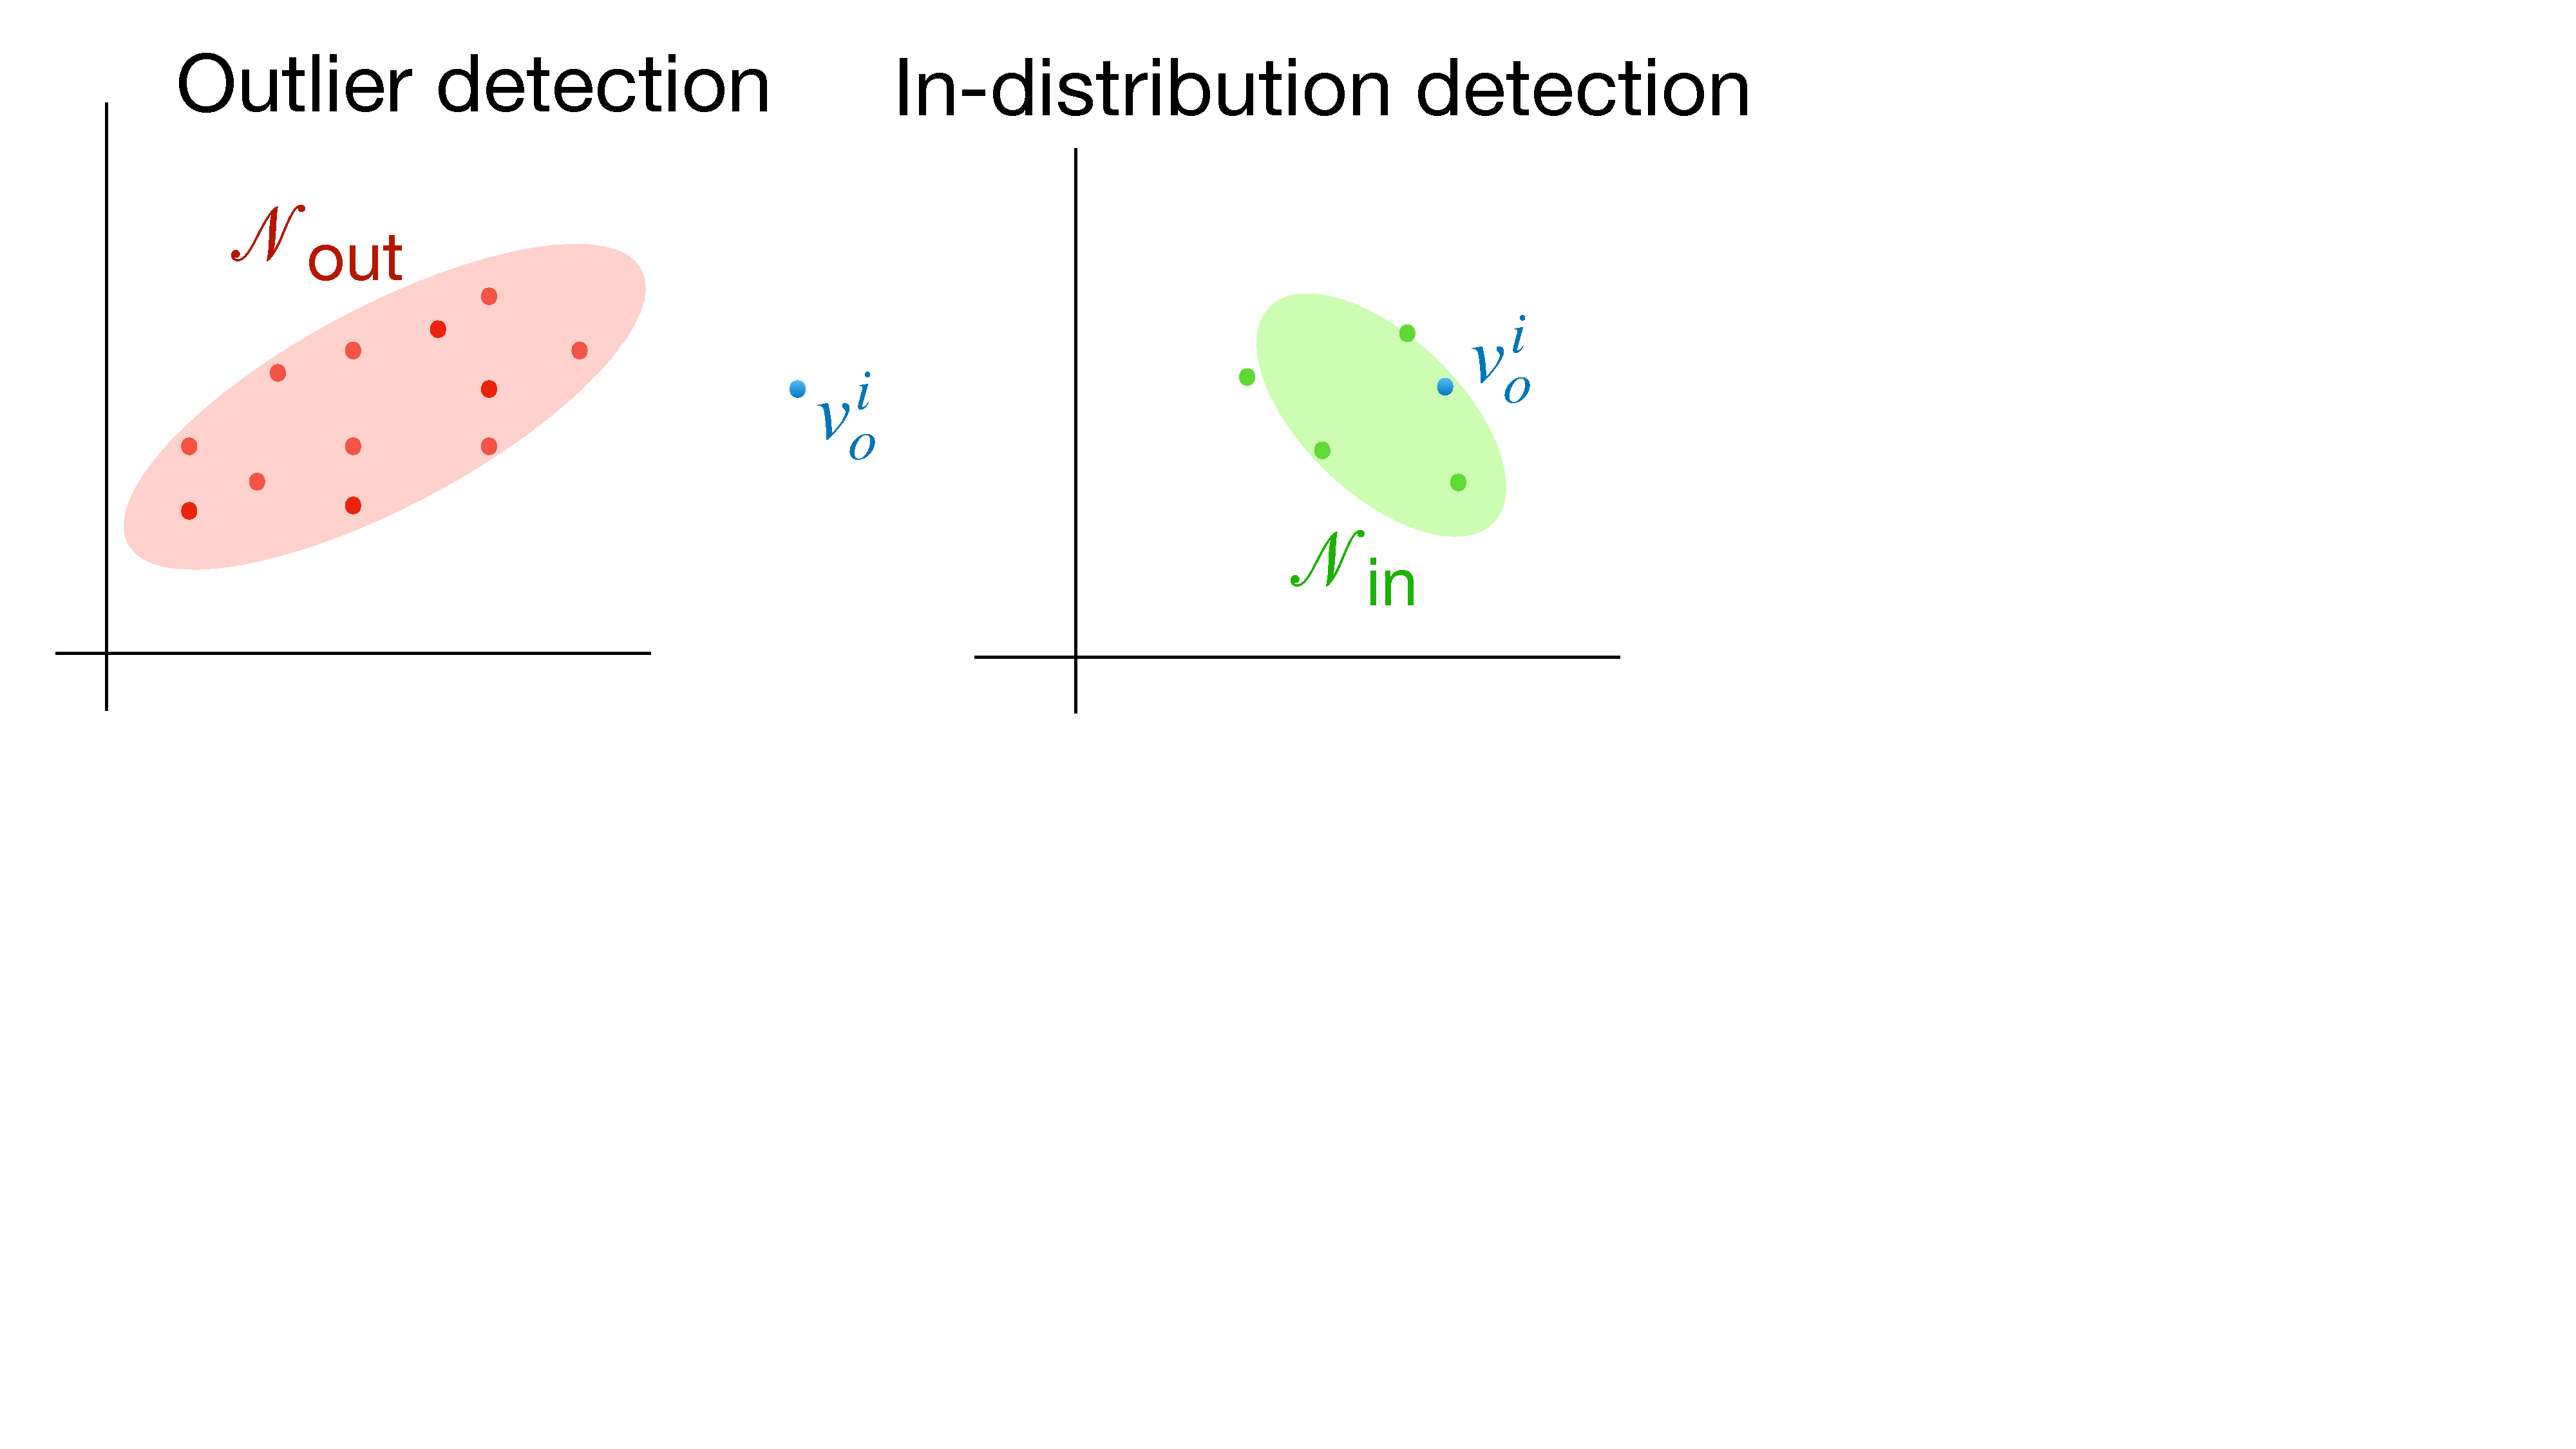
\includegraphics[width=0.9\columnwidth]{submissions/Ali2023/figures/outin.pdf}
      \caption{Two formulations for fact verification. Outlier detection samples a pool of non-existing facts and prioritizes objects that are outliers (left); in-distribution detection samples a pool of existing facts and prioritizes facts that are in-distribution samples to the pool (right).}
    \label{fig:met_out}
\end{figure}


\subsection{Out-of-distribution Sample Detection}
% \paragraph{Out-of-distribution sample detection non-existing facts with same head entity $v_s^i$ and relation $r_i$}
The first method considers a pool of non-existing facts with the same subject entity $v_s^i$ and relation $r^i$ as the related facts for the triplet $(v_s^i, r^i, v_o^i)$ in $\gE_\text{V}$.
We can formulate fact verification---especially verification of facts that might be missing---as an out-of-distribution sample detection task.
We can score the triplet $(v_s^i, r^i, v_o^i)$ by checking whether this is an ``outlier'' to the pool of non-existing facts. If it is an outlier, we may prioritize this triplet fact since it is more likely to be a True missing fact.
For each triplet in the given set of triplets $\gE_\text{V}: \{(v_s^1, r^1, v_o^1), \dots, (v_s^n, r^n, v_o^n)\}$, we score it in the following way against a set of related non-existing facts:
In order to score $(v_s^i, r^i, v_o^i)$, we first construct non-existing facts by replacing the objects of the query $(v_s^i, r^i, ?)$. We sample entities $v$ from KG as the object if $(v_s^i, r^i, v) \notin \gE$ using importance sampling, where the weight of each non-existing fact is proportional to the distance $p_{(v_s^i, r^i, v)}\propto\exp({\distt{v_s^i}{r^i}{v}})$ since we would like to sample non-existing facts with high confidence measured by the learned embeddings.
% Note this is sufficient in our use case and achieves empirically nice experimental results (detailed in \Secref{sec:ali_experiment}), but one could design better negative sampling strategies \tocite{} to further improve fact pool. 
Assume we sample a pool of $k$ non-existing facts for the $i$-th triplet $(v_s^i, r^i, v_o^i)$, $\gP^i_\text{NE}: \{(v_s^i, r^i, v_1), \dots, (v_s^i, r^i, v_k)\}$ as well as the triplet fact $(v_s^i, r^i, v_o^i)$ to verify, we measure the delta using Mahalanobis distance-based confidence score. In detail, we estimate the mean and covariance of the entity embeddings of these negative samples $v_1, \dots, v_k$:
\begin{align}
    \vmu_\text{out}&=\frac{1}{k} \sum_j f_\theta(v_j) \nonumber\\
    \mSigma_\text{out}&=\frac{1}{k} \sum_j (f_\theta(v_j) - \vmu)(f_\theta(v_j) - \vmu)^\intercal,\label{eq:distribution_out}
\end{align}
which is the maximum likelihood estimation of the parameters of the multi-variate Gaussian distribution $\gN_\text{out}$.
We define the score $s_i$ of $(v_s^i, r^i, v_o^i)$ using the Mahalanobis distance between the embedding of and the Gaussian distribution $\gN_\text{out}$:
\begin{align}
    s_i = (f_\theta(v_o^i) - \vmu_\text{out})^\intercal \mSigma^{-1}_\text{out}(f_\theta(v_o^i) - \vmu_\text{out}).\label{eq:score_out}
\end{align}
Since large-scale KGs are often extremely sparse, we can easily construct a pool of $k$ non-existing facts with $k>1000$. In such a way, we can have an accurate estimation of the distribution $\gN_\text{out}$.
In order to identify the promising triplet facts, we formulate the problem as a binary classification task using the $s_i$, and prioritize ones with large $s_i$, which means that they are far from the $\vmu_\text{out}$ and likely to be a missing fact.

\subsection{In-distribution Sample Detection}
% \paragraph{Existing facts with same subject entity $v_s^i$ and relation $r_i$}
We can also approach the problem from the opposite perspective. Instead of scoring the fact $(v_s^i, r^i, v_o^i)$ using a set of related non-existing facts, we can score it using a set of existing facts with the same subject entity $v_s^i$ and relation $r^i$.  
For a given $(v_s^i, r^i, v_o^i)$, we find all answers $\gA_q$ to query $q=(v_s^i, r^i, ?)$ in the KG, and define the pool of related triple facts to be $\gP^i_\text{E}: \{(v_s^i, r^i, v_1), \dots, (v_s^i, r^i, v_k)\}$, where $v_1, \dots, v_k\in\gA_q$. 
Similarly, we can estimate a multivariate Gaussian distribution $\gN_\text{in}$:
\begin{align}
    \vmu_\text{in}&=\frac{1}{k} \sum_j f_\theta(v_j) \nonumber\\
    \mSigma_\text{in}&=\frac{1}{k} \sum_j (f_\theta(v_j) - \vmu)(f_\theta(v_j) - \vmu)^\intercal.\label{eq:distribution_in}
\end{align}
We define the score $s_i$ of $(v_s^i, r^i, v_o^i)$ using the Mahalanobis distance between the embedding of $v_o^i$ and the Gaussian distribution $\gN_\text{in}$:
\begin{align}
    s_i = (f_\theta(v_o^i) - \vmu_\text{in})^\intercal \mSigma^{-1}_\text{in}(f_\theta(v_o^i) - \vmu_\text{in}).\label{eq:score_in}
\end{align}
Since the pool of related facts are existing facts on the graph, we need to identify triplets with small score, which means that they are an in-distribution sample of the pool.
The key challenge of this method is that the estimation has high variance due to the limited number of answer size $|\gA_q|$. For example, the average number of answers for predicate \texttt{OccupationOf} is 1.32 in Wikidata. 

To improve the estimation accuracy we loosen the definition of related triple facts for $(v_s^i, r^i, v_o^i)$ by finding entities $v$ that are close to the subject entity $v_s^i$ in the embedding space. The intuition is that entities that are close in the embedding space share similar semantic meaning, \eg, the neighbors obtained by the Query2Box model for `Selena Gomez' node are all singer entities: including the nodes corresponding to `Taylor Swift', `50 Cent', `Miley Cyrus', `Halsey', and `Jay-Z'. Assume we find $m$ close entities of $v_s^i$: $\{v_1, \dots, v_m\}$, we collect the pool of existing related facts as the \emph{union} of all the triplet with one of the close entities as the subject and the relation of interest $r^i$ as the relation type, \ie, $\gP^i_\text{U}: \cup_{j=1}^m\:\{(v_j, r^i, v) | v\in\gA_q, q=(v_j, r^i, ?)\}$. 
We can tune the parameter $m$ to achieve a balance between computation efficiency and the accuracy of the estimation.
However, here we cannot simply use the previous framework, \ie, we cannot aggregate all the object entities in the pool and estimate the mean and covariance matrix only using the embeddings of the object entities as in \eqref{eq:distribution_in} and \eqref{eq:score_in}. The reason is that (1) there may be overlapping object entities, \ie, there exists an entity $v_\text{object}$ that is the object to multiple subject entities in the $\gP^i_\text{U}$, \ie, $\exists v_\text{object}, v_\text{subject}^1 \neq v_\text{subject}^2, \: (v_\text{subject}^1, r^i, v_\text{object}) \in \gP^i_\text{U}$ and $(v_\text{subject}^2, r^i, v_\text{object}) \in \gP^i_\text{U}$; (2) since the subject entities are different in the pool $\gP^i_\text{U}$, we need to \emph{align} the object entity $v_\text{object}$ with the subject entity $v_\text{subject}$ given a $(v_\text{subject}, r^i, v_\text{object})$ in the pool $\gP^i_\text{U}$. 

\begin{figure}
        \centering
      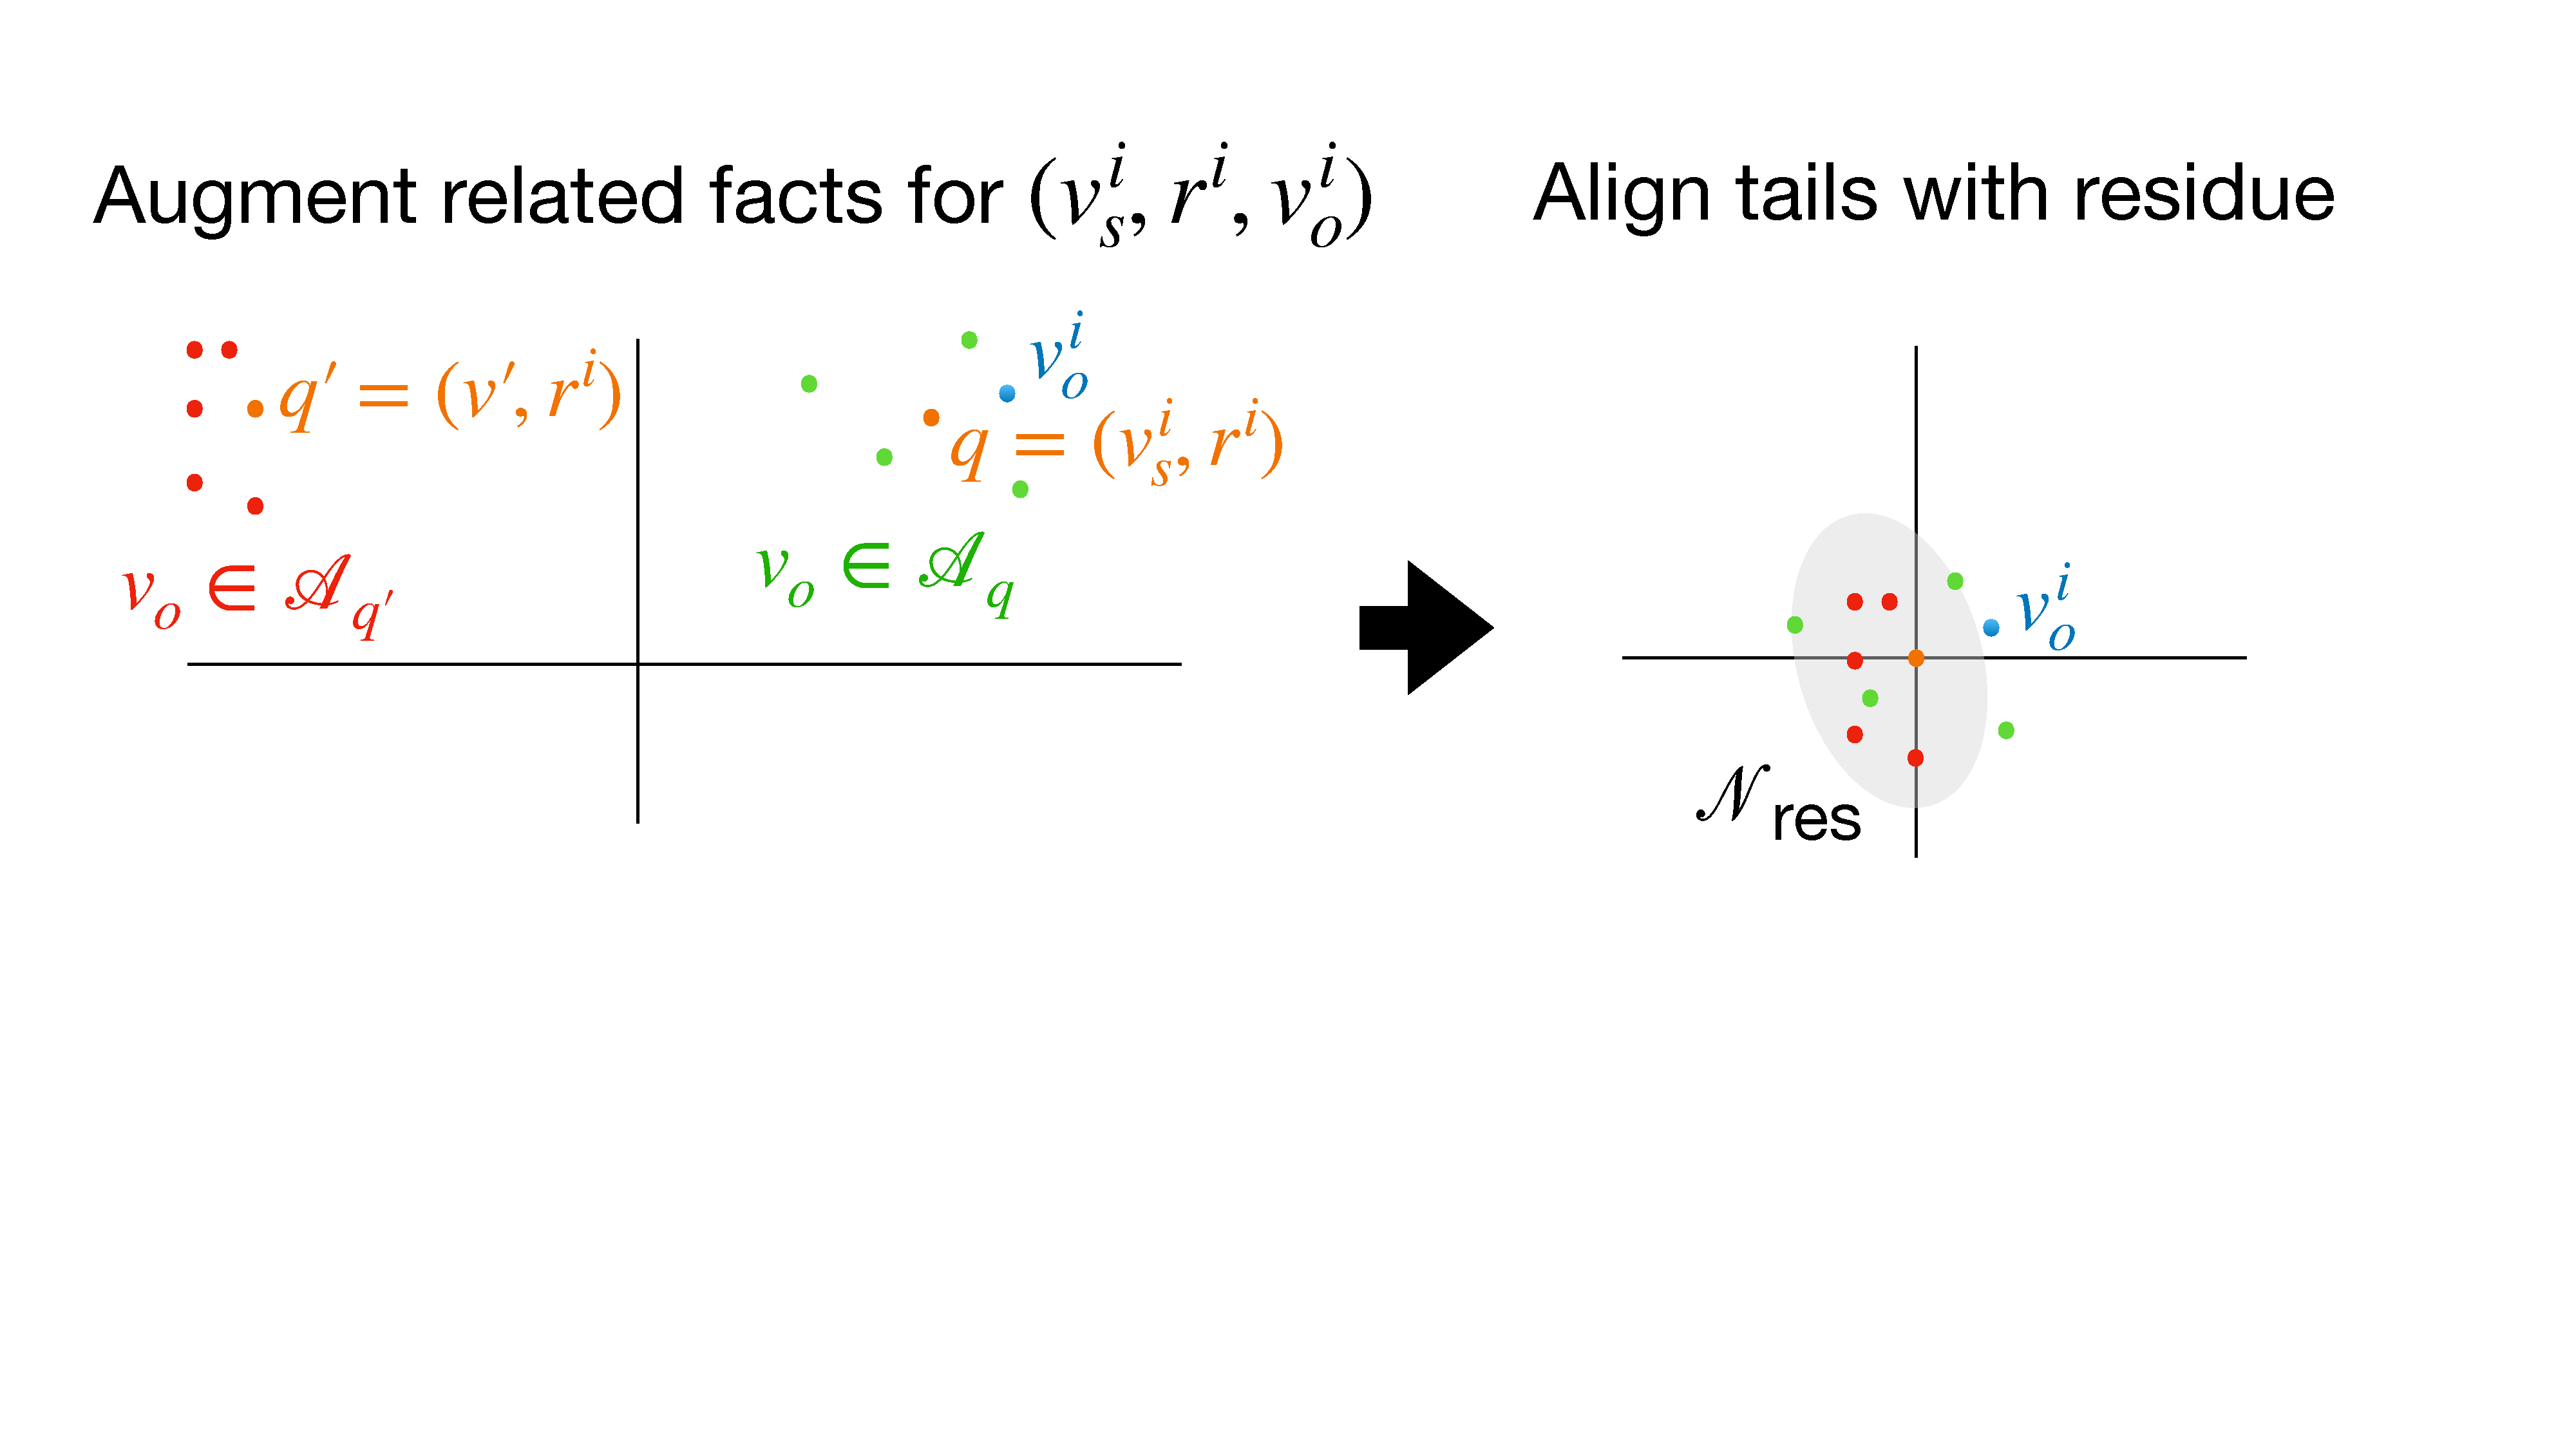
\includegraphics[width=\columnwidth]{submissions/Ali2023/figures/residue.pdf}
      \caption{In the in-distribution sample detection method, for a given fact $(v_s^i, r^i, v_o^i)$, we augment the pool of related facts by including facts with similar subject entities and the same relation $r^i$. As shown in the left Figure, we also consider facts $\{(v', r^i, v_o)\:|\:v_o\in\gA_q', q'=(v', r^i)\}$ as related facts. We align the object embeddings by finding the residue and estimate the $\gN_\text{res}$. We finally check whether the object $v_o^i$ is an in-distribution sample from $\gN_\text{res}$.}
    \label{fig:residue}
\end{figure}

Inspired by product quantization~\cite{jegou2010product}, here we align the object embedding by finding the residue between the query, \ie, the (subject, relation) pair $(v_\text{subject}, r^i)$ and the object entity $v_\text{object}$. Since the entity embeddings are high dimensional, the goal of this residue function is to capture the difference between the query and object \emph{along each dimension}. Different KG embedding methods may have different residue functions. Below we show the residue function of TransE with L1 distance for example.
\begin{align}
    \texttt{Residue}(v_s, r, v_o) = f_\theta(v_s) + f_\theta(r) - f_\theta(v_o).\label{eq:residue}
\end{align}
We emphasize that the residue function is different from the distance function in \eqref{eq:kgelossfunc}. The output of the residue function is a high-dimensional vector that represents the difference between a subject-relation pair and an object along each dimension, while \texttt{Dist} outputs a scalar distance.

Now given the related existing fact pool $\gP^i_\text{U}$ for triplet fact $(v_s^i, r^i, v_o^i)$, we first calculate the residue for each related fact in the pool: $\mathcal{S}^i_\text{U}: \{\texttt{Residue}(v_\text{subject}, r^i, v_\text{object}) | (v_\text{subject}, r^i, v_\text{object})\in\gP^i_\text{U}\}$, and then fit a multi-variate Gaussian distribution $\gN_\text{res}$:
\begin{align}
    \vmu_\text{res}&=\frac{1}{|\mathcal{S}^i_\text{U}|} \sum_{\vx\in\mathcal{S}^i_\text{U}} \vx \nonumber\\
    \mSigma_\text{res}&=\frac{1}{|\mathcal{S}^i_\text{U}|} \sum_{\vx\in\mathcal{S}^i_\text{U}} (\vx - \vmu)(\vx - \vmu)^\intercal.\label{eq:distribution_res}
\end{align}
Then we define the score $s_i$ using the Mahalanobis distance between the residue of $(v_s^i, r^i, v_o^i)$ and the Gaussian distribution $\gN_\text{res}$:
\begin{align}
    s_i = (\distr{v_s^i}{r^i}{v_o^i} - \vmu_\text{res})^\intercal \mSigma^{-1}_\text{res}(\distr{v_s^i}{r^i}{v_o^i} - \vmu_\text{res}).\label{eq:score_res}
\end{align}
We can prioritize facts with small $s_i$: although these facts do not exist in the graph, they are close to existing facts, so we should have human curators to verify these facts first.

\subsection{Distance Compared with Related Facts}
Besides the formulations of out-of-distribution/in-distribution sample detection, we also design a simple method that directly score the triplet $(v_s^i, r^i, v_o^i)$ by modeling the difference of the absolute distance of $(v_s^i, r^i, v_o^i)$ and the related facts.
Here we may reuse the definition of related facts as in previous sections, including non-existing facts with the same $v_s^i$ and relation $r^i$ as subject and relation, or existing facts with close subject entities and relation $r^i$.

Consider that we sample $k$ non-existing facts for the $i$-th triplet $(v_s^i, r^i, v_o^i)$: $\gP^i: \{(v_s^i, r^i, v_1), \dots, (v_s^i, r^i, v_k)\}$ as well as the triplet fact $(v_s^i, r^i, v_o^i)$ to verify, we formulate and measure the delta using the distance calculated by the embeddings. We calculate the distance $d_1=\distt{v_s^i}{r^i}{v_1}\in\R, \dots, d_k$, together with $d_t=\distt{v_s^i}{r^i}{v_o^i}$, and measure how $d_t$ is compared against $\{d_1, \dots, d_k\}$. We estimate a Gaussian distribution $\gN_\text{D}=(\mu_\text{D}, \sigma_\text{D})$ over the distances of non-existing facts $\{d_1, \dots, d_k\}$, and score $(v_s^i, r^i, v_o^i)$ by calculating how many standard deviations $d_t$ are away from the mean: $s_i=\frac{d_t - \mu_\text{D}}{\sigma_\text{D}}$. Here in order to identify the promising triplet facts, we prioritize ones with small $s_i$, which means that the distance of $(v_s^i, r^i, v_o^i)$ is considered much smaller than that of the related facts (estimated using $\gN_\text{D}$) and thus the triplet is likely to be a missing fact.

\subsection{Application to Verification of Existing Facts}
Above we introduced how we use our framework to solve one of the fact verification tasks, namely identifying the likely missing triplet facts. Another task that falls within the same domain is that we want to prioritize the existing triplet facts on the graph that are likely to be False. Our framework can be naturally adapted for this setting, where we can still collect related triplet facts, do outlier / in-distribution sample detection, or estimate a distribution of distance, and calculate how many standard deviations is this triplet fact away from the mean. Then we can use this score to identify and prioritize promising triplet facts in this setting.

\fi